\documentclass{article}

\usepackage{amsmath}
\usepackage{amsthm}
\usepackage{amssymb}
\usepackage{float}
\usepackage{graphicx}
\usepackage{subfig}
\usepackage[utf8]{inputenc}
\usepackage[english]{babel}
\usepackage[linesnumbered,ruled]{algorithm2e}

\theoremstyle{definition}
\newtheorem{definition}{Definition}[section]
\newtheorem{theorem}{Theorem}

\title{%
	Logical Neural Networks: Opening the black box\\
	\large Logical Normal Form Network
}
\author{Daniel Braithwaite}

\begin{document}

\maketitle

Given a simple feed foward network using neurons resembleing NAND gates is unable to learn any given boolean formula we switch our interest to something else. We know that any boolean expression can be represented in Conjunctive Normal Form (CNF) or Disjunctive Normal Form (DNF). So it seems prudent to ask wether its possible to construct a feedfoward netural netowrk which can learn these underlying representations. Findings \cite{herrmann1996backpropagation} seem to sugest that it is possible however there is limited justification for some claims and because of this is diffcult to reproduce. We will take this general concept and reproduce the research in an attempt to develop a better understanding.

\section{Noisy Neurons}
During a previous investigation of Logical Neural Networks the concept of Noisy-OR and Noisy-AND neurons where derived \cite{LearningLogicalActivations}. Here we will simply state them as.

\theoremstyle{definition}
\begin{definition}{}
A \textbf{Noisy-OR} neuron is a perceptron with activation $a = 1 - e^{-z}$ where $W$ is our weights, $X$ is our inputs, $b$ is our byas term and $z = WX + b$. We contrain each $w_i \in W$ and b to be in the interval $[0, \inf]$
\end{definition}

\begin{definition}{}
A \textbf{Noisy-OR} neuron is a perceptron with activation $a = e^{-z}$ where $W$ is our weights, $X$ is our inputs, $b$ is our byas term and $z = WX + b$. We contrain each $w_i \in W$ and b to be in the interval $[0, \inf]$
\end{definition}

\section{Logical Normal Form Networks}
A Logical Normal Form Network is a neural net which stasfys one of the folowing definitions

\theoremstyle{definition}
\begin{definition}{CNF-Network}
A \textbf{CNF-Network} is a three layer network where neurons in the hidden layer consist soley of Noisy-OR's and the output layer is a single Noisy-AND. 
\end{definition}

\theoremstyle{definition}
\begin{definition}{DNF-Network}
A \textbf{DNF-Network} is a three layer network where neurons in the hidden layer consist soley of Noisy-AND's and the output layer is a single Noisy-OR. 
\end{definition}

It is worth noteing that CNF and DNF form can have the nots of atoms in there clauses, a simple way to account for this is to double the number of inputs where one represents the atom and the next represents the negation of that atom.

\subsection{Learnability Of Boolean Gates}
Theoretiaclly it makes sense for these networks to be able to learn the CNF and DNF representations of various boolean expressions, however before we attempt arbatary boolean functions we would like to start with something simple, namely expressions such as NOT, AND, NOR, NAND, XOR and IMPLIES. Results of which where promising, we where able to achieve a low error and from inspecting the weights we could see that the networks where infact learning the correct CNF and DNF representations.\\

\subsection{Learnability Of Interesting Expressions}
We now wish to see if we can use these networks to learn more interesting boolean formula, starting with expressions of 3 variables. While we are able to achieve a small error there is now some noise (i.e. small non zero weights for inputs that are irrelevant). While a small ammount of noise is okay and can be pruned out after training we could run into issues if the ammount of noise increases as the number of inputs does. \\

One other interesting observation to be made is that both the CNF and DNF Netoworks have trouble learning the boolean expression $(a\ XOR\ b)\ AND\ c$. They can't achevice an error lower than 1. Indivually we can learn an XOR gate and an AND gate but somehow combining the two results in something which is unlearnable.\\

During the investigation of this a more sinister issue was uncovered, namely that these LNF netowrks are unable to learn boolean expressions of 2 variables when given 3. I.e. we give the network all values for three inputs, a, b and c but we only want to learn $a\ OR\ b$. This is a fundimental issue as in practice most problems will be made up of boolean expressions which dont rely on all inputs. \\

It turns out this problem was not caused by a problem with our LNF Networks but with the weight initilizations, namely they where currently initilised to 0, changing the weights to be randomly distrubuted over the interval [0,1] fixed this problem and allows the LNF Networks to solve all attempted problems so far, along with there weight representations being intepretable. However the networks seem quite sensitive to there intial conditions, an investgation of best ways to initilise LNF networks would be prudent.

\section{LNF Network Learning Issues}
Before we can hope to compare peformance, pruning or generalization we must address an issue with learning boolean functions of size 7 or greater.

\begin{figure}[H]
\centering
  \begin{minipage}[b]{0.4\textwidth}
    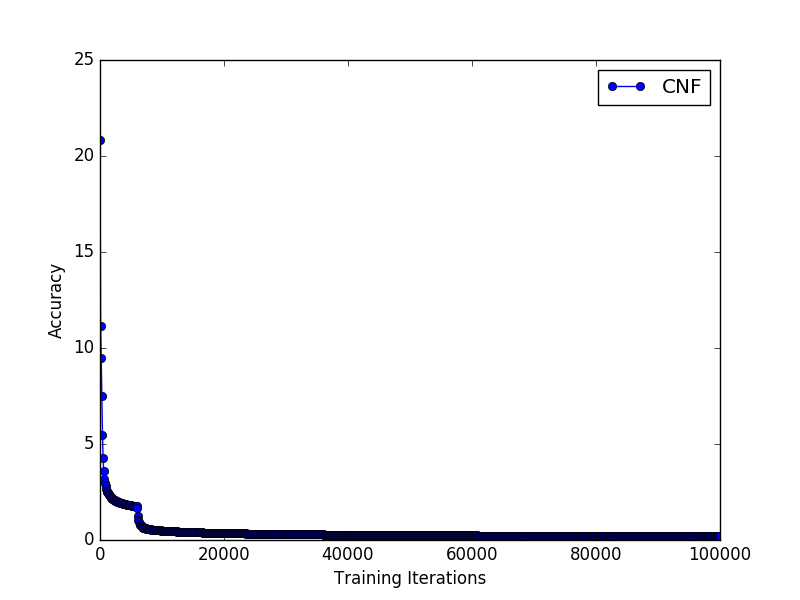
\includegraphics[width=\textwidth]{CNF-LD-iterations.png}
    \caption{Boolean Formula of size 6}
  \end{minipage}
  \hfill
  \begin{minipage}[b]{0.4\textwidth}
    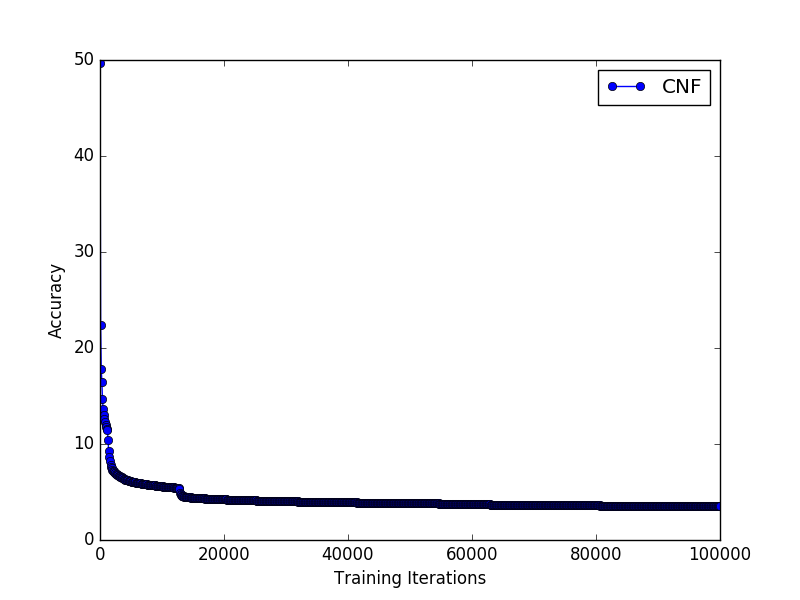
\includegraphics[width=\textwidth]{CNF-LD2-iterations.png}
    \caption{Boolean Formula of size 7}
  \end{minipage}
\end{figure}

The above graphs demonstraite a CNF Network learning boolean formulas of size 6 and 7. As we move from 6 to 7 we are unable to achieve an error close enough to 0. As we further increase N this only gets worse. Here we will explore possible options for how to fix this

\subsection{Weight Initilization}
Currently the weights are initilized from the uniform distrubution $[0,1]$, however one noticible feature of trained networks of lower inputs is that the weights which noise (i.e. once removed reveal the CNF or DNF of the formula) are in the interval $[0,1]$. Trying different intervals for initilizing the weights could result in better peformance.

\begin{figure}[H]
\centering
  \begin{minipage}[b]{0.4\textwidth}
    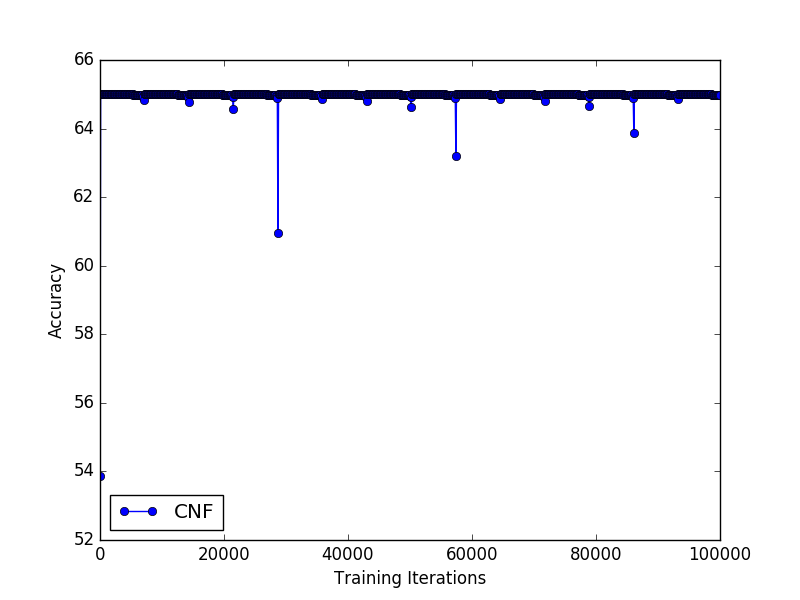
\includegraphics[width=\textwidth]{CNF-LD-WI-01.png}
    \caption{Weight initilization from uniform in [1.0, 3.0]}
  \end{minipage}
  \hfill
  \begin{minipage}[b]{0.4\textwidth}
    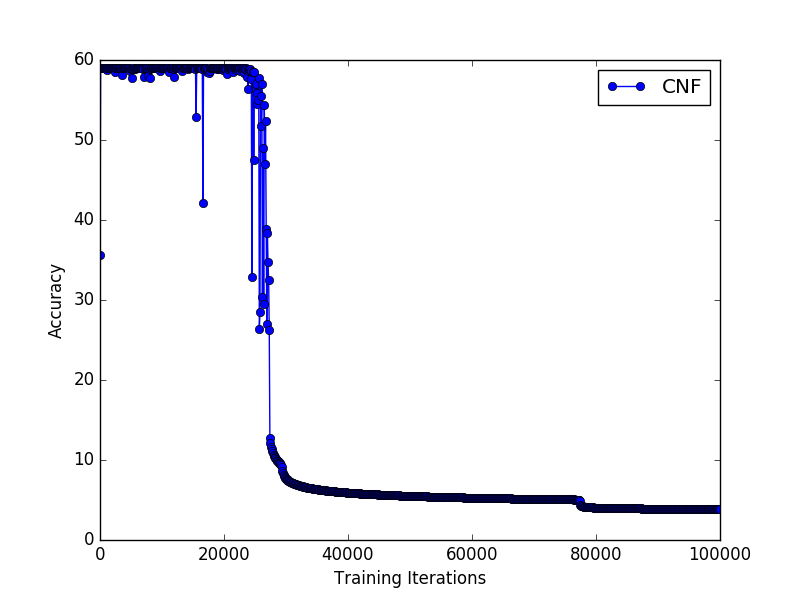
\includegraphics[width=\textwidth]{CNF-LD-WI-02.png}
    \caption{Weight initilization from uniform in [0.5, 1.5]}
  \end{minipage}
\begin{minipage}[b]{0.4\textwidth}
    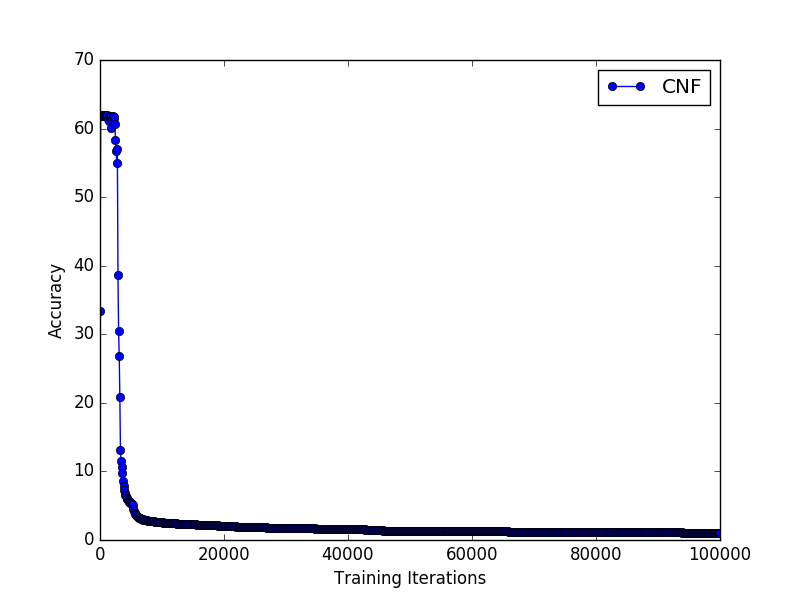
\includegraphics[width=\textwidth]{CNF-LD-WI-03.png}
    \caption{Weight initilization from uniform in [0.0, 2.0]}
  \end{minipage}
\end{figure}

This significantly improves the peformance of learning boolean functions of 7 inputs for learning all boolean functions of less that 7 inputs aswell. Does further increasing the upper bound on this initilization range keep increasing the peformance? Also does this change in initilization range fix the similar problems with boolean functions of size greater than 7?

\begin{figure}[H]
\centering
  \begin{minipage}[b]{0.4\textwidth}
    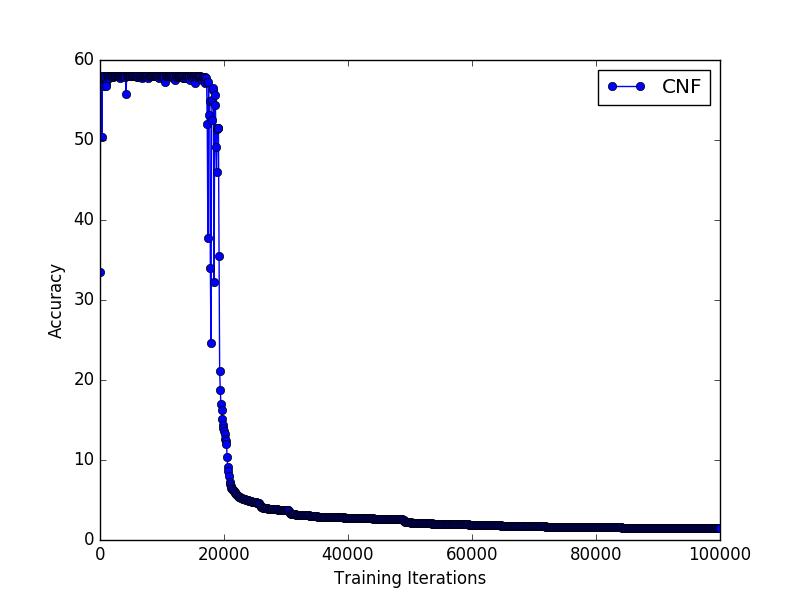
\includegraphics[width=\textwidth]{CNF-LD-WI-04.png}
    \caption{Weight initilization from uniform in [0.0, 3.0]}
  \end{minipage}
  \hfill
\end{figure}

So further increasing the range does not help peformance. Also our current change dosnt benifit when we move to functions of size 8

\begin{figure}[H]
\centering
  \begin{minipage}[b]{0.4\textwidth}
    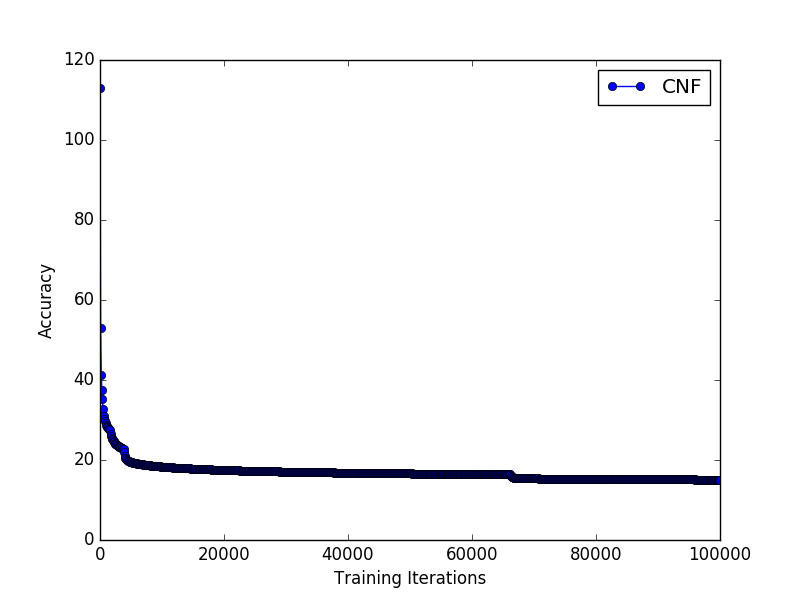
\includegraphics[width=\textwidth]{CNF-LD-WI-06.png}
    \caption{Size 8 Weight initilization from uniform in [0.0, 1.0]}
  \end{minipage}
  \hfill
  \begin{minipage}[b]{0.4\textwidth}
    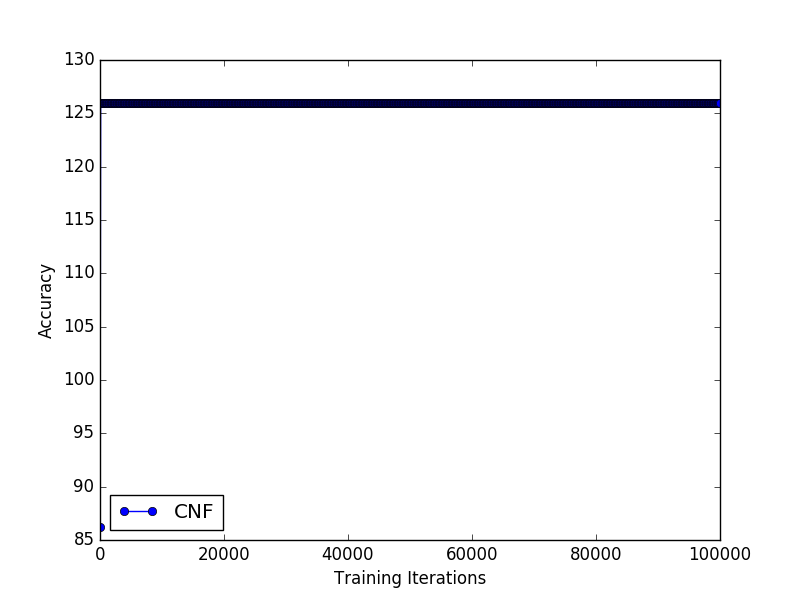
\includegraphics[width=\textwidth]{CNF-LD-WI-05.png}
    \caption{Weight initilization from uniform in [0.0, 2.0]}
  \end{minipage}
\end{figure}

\subsection{Different Optimizers}
Currently we are using Gradient Descent to optimize our paramaters, however there are other optimization techequics that could be more suitible our networks. Such as Adam or RMSProp.

\begin{figure}[H]
\centering
  \begin{minipage}[b]{0.4\textwidth}
    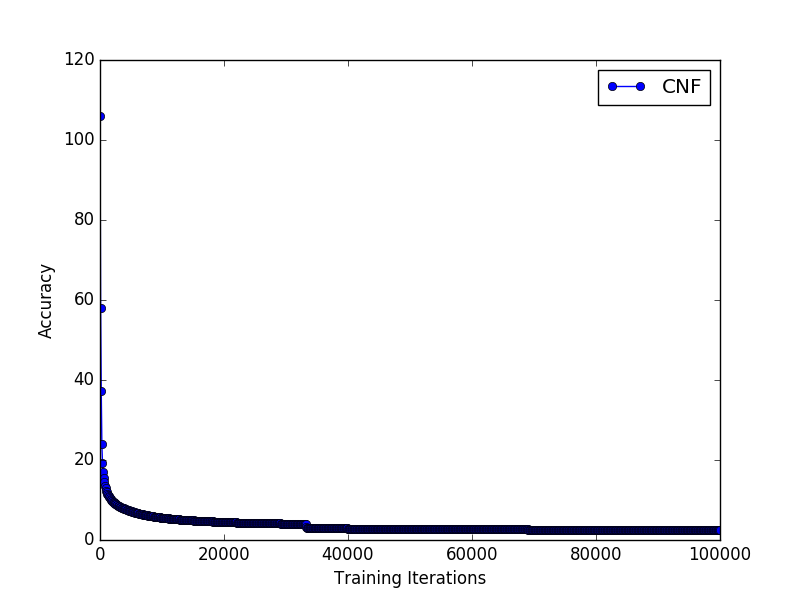
\includegraphics[width=\textwidth]{CNF-OP-ADAM-01.png}
    \caption{Size 8 With ADAM optimizer}
  \end{minipage}
  \hfill
  \begin{minipage}[b]{0.4\textwidth}
    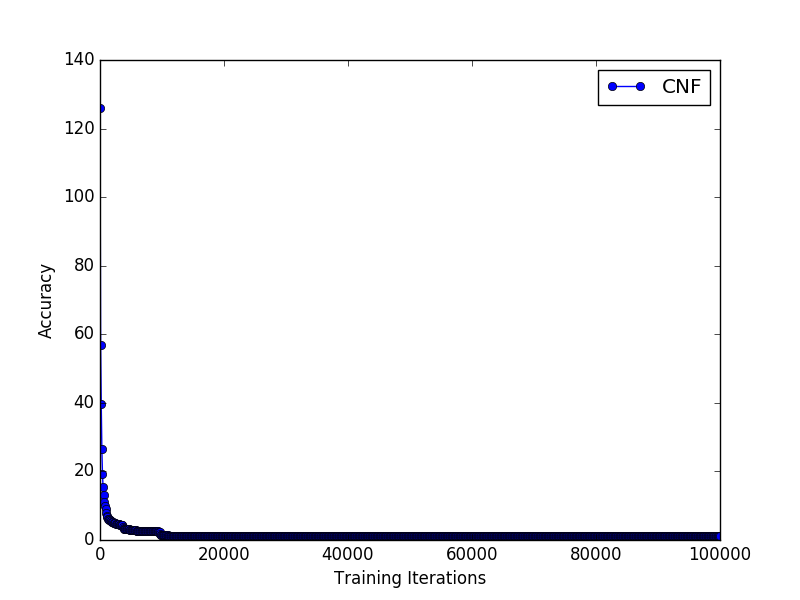
\includegraphics[width=\textwidth]{CNF-OP-RMS-01.png}
    \caption{Size 8 With RMS optimizer}
  \end{minipage}
\end{figure}

RMSProp gives us signigicant improvement at 8 inputs, but are we able to maintain this improvement while we scale up the number of inputs? From experementation as we increase the number of inputs we need a smaller learning rate to achieve a smalle error. This means the larger the number of inputs the larger the training time required, as demonstraited below

\begin{figure}[H]
\centering
  \begin{minipage}[b]{0.4\textwidth}
    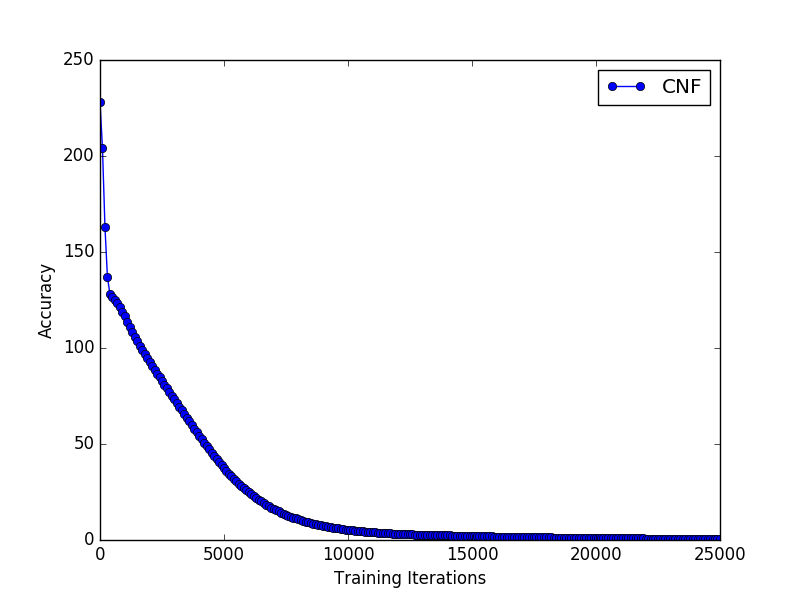
\includegraphics[width=\textwidth]{CNF-OP-RMS-03.png}
    \caption{RMSProp with size 9, learning rate 0.0005 and total iterations 20000. Error 0.5}
  \end{minipage}
  \hfill
  \begin{minipage}[b]{0.4\textwidth}
    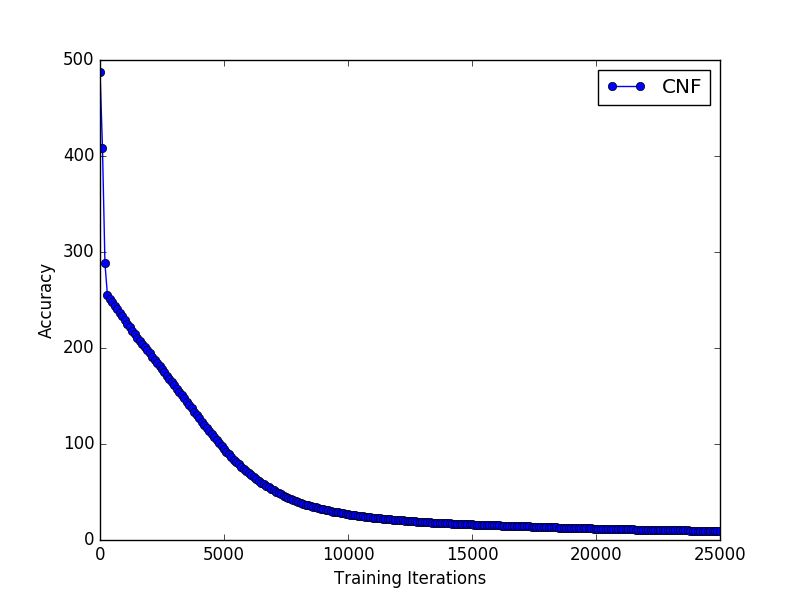
\includegraphics[width=\textwidth]{CNF-OP-RMS-04.png}
    \caption{RMSProp with size 10, learning rate 0.0005 and total iterations 25000. Error 9.5}
  \end{minipage}
\end{figure}

However these expressions are still not correct, even at n=4 we are able to achieve a low error but we cant extract the correct CNF formula. To make the error easier to intepret we will switch to using the cross entropy loss. We now observe that when training on 4 inputs we achieve an error of 1.1 but when we extract our formula we find we are getting 4 of the input patterns wrong. This indicates that our Noisy-OR and Noisy-AND neurons arnt restrictive enough and allow solutions which dont corospond to an OR or AND operation. So we need to choose a different paramaterisation for our CNF and DNF Networks.

\subsection{Regularisation}
Esentially we know that there exsists a weight representation that corosponds to a boolean formula, to encourage our network to learn this representaton we will use regulrization on the weights. Esentially we want to reward the network for having weights which are either 0 or really large, it is not immeaditly obvious how to reward the network for this so to simplyfy things we can switch to our Noisy-OR, Noisy-AND represented which has bounded weights.\\

Using this bounded weight representation also removes the decision of the range to initilize over as now we can uniformly distrubute over the entire range.\\

Now we know that all our weights will be in the interval $[0, 1]$ meaning we can use a 1D-Gussian function as our penalty, which has the nice property allowing us to adjust the seapness. The generic function, where $\beta$ defines our steepness.

\begin{align}
p(w) = e^{-\beta (w - 0.5)^2}
\end{align}

Purely by abrtrary decision and from inspecting graphs we choose to use $\beta = 25$. Now we can make our regulrization the sum over all weights, $\lambda \sum p(w)$. We should note that we do not regurilize on the biases, these can take on any value in the interval $[0,1]$ as we dont take these into account when deciding what variables a Noisy neuron is considering.

We denote these networks as \textbf{Binary LNF Networks}, as once trained, if there is a boolean formula to be learnt then the weights will be binary.

\section{Dicussion}
Using our regularisation technequic not only are we able to achieve better results but given that our networks are now binary at the conclusion of training we are also able to extract boolean formula from these networks which when run over the binary inputs and outputs get 100\% accuracy. This is testing up to boolean formulas of 7 inputs, previously we where unable to get consistant results on size 3, letalone get any good results on 7. There is however alot of blote in these formulas, many clauses in the formula are tautologies, i.e. always true. \\

After trying both on and offline training I found that the best and most consistant results where achieved with online. This makes intuitive sense as we expect that each neuron will respond positively to a subset of the training data.\\

However time taken to train these networks is now a significant factor, one reason is that of online learning, effort must now be put into speeding up the training time otherwise these LNF Networks are not feasable in practice.

\section{Binary LNF Network Training Time}
In this section we hope to work toward reducing the time taken to train our models, currently implemented in TensorFlow which is significantly faster than vanalla python however we need further increase in peformance.

\section{LNF Network Peformance}
We wish to compare the CNF and DNF networks against each other but also against standard perceptron networks. We will take 5 randomly choosen boolean expressions of n inputs for n between 2 and 10. For each we will train CNF, DNF and Perceptron networks 5 separate times and use the datapoints to peform significance tests between the three.

\section{LNF Network Generalization}
Say we are trying to learn a boolean function of $n$ inputs, we know for a fact there are $2^n$ total input patterns in total for this boolean function. We also know there are $2^n$ total possible boolean functions with $n$ inputs. So an important question to ask is once we start to remove some of the traning examples what happens to our network accuracy? The usefulness of standard neural networks is in part because they are able to take a sample of the total data set and then generalise well to unseen examples, can we achieve the same with LNF networks?\\

We will take one boolean expression with $n = 4$ and slowley remove from the pool of traning examples, training a fresh network each time. This will allow us to see a trend of network accuracy as we remove more and more from the training pool.

\section{LNF Network Rule Extraction}

\subsection{LNF Network Pruning}


\medskip
\bibliographystyle{acm}
\bibliography{bibliography}
\end{document}